\documentclass{article}
\usepackage{setspace}
\usepackage{graphicx}
\usepackage{float}
\usepackage{chngpage}
\usepackage{subcaption}
\usepackage{framed}
\usepackage{listings}
\graphicspath{ {./media/} }
\usepackage[backend=biber, style=authoryear-icomp,doi=false,isbn=false,url=false]{biblatex}
\addbibresource{$BIB}

\definecolor{codegreen}{rgb}{0,0.6,0}
\definecolor{codegray}{rgb}{0.5,0.5,0.5}
\definecolor{codepurple}{rgb}{0.58,0,0.82}
\definecolor{backcolour}{rgb}{0.95,0.95,0.92}

\lstdefinestyle{mystyle}{
    backgroundcolor=\color{backcolour},
    commentstyle=\color{codegreen},
    keywordstyle=\color{magenta},
    numberstyle=\scriptsize\color{codegray},
    stringstyle=\color{codepurple},
    basicstyle=\ttfamily\scriptsize,
    breakatwhitespace=false,
    breaklines=true,
    captionpos=b,
    keepspaces=true,
    numbers=left,
    numbersep=5pt,
    showspaces=false,
    showstringspaces=false,
    showtabs=false,
    tabsize=2
}
\lstset{style=mystyle}

\addtolength{\oddsidemargin}{-.5in}
\addtolength{\evensidemargin}{-.5in}
\addtolength{\textwidth}{1in}
\addtolength{\topmargin}{-.5in}
\addtolength{\textheight}{1in}

\newenvironment{centerfig}
{\begin{figure}[H]\centering}
{\end{figure}}




\begin{document}
\title{}
\maketitle{}
\textit{This paper uses Google search terms containing offensive language as a proxy measure for racial animus. Following the practice of similar works \parencites{Stephens_Davidowitz_2014}{Chae_2015}{Chae_2018}{Isoya_2021}, I use coded language to refer to these terms. The words themselves can be found in Table \ref{words}}

\section{Introduction}

\section{Methods}

\subsection{Tools Used}

Surveys of major social science journals routinely fail to reproduce the findings of a plurality or majority of published articles, even when using data provided with the paper \parencites[][]{Nuijten_2015}{Nuijten_2020}{Eubank_2016}.
In many cases, failures to replicate are due to coding errors or mistakes in transcribing the results of a calculation into the published manuscript \parencite[][]{Eubank_2016}.

To ensure that the methods of this paper have been properly implemented and the finding are reproducible, I tested the analysis routines using the \textit{testthat} package in R \parencite[][]{testthat} and the \textit{unittest} module in Python \parencite[][]{Python}.
I use Kintr to integrate statistical calculations into the paper, eliminating the possibility of transcription errors \parencite[][]{knitr}.

Finally, I provide a Docker image \parencite[][]{docker} with the reproducibility materials to ensure others can replicate the figures in this paper on their own systems \parencite{Boettiger_2015}.
The net result is ``one-click reproducibility" \parencite[][]{N_st_2020}; readers can reproduce this exact paper with the push of a button on their own systems from the reproducibility materials.


\begin{figure}
\caption{Sinclair News Anchors Reading a ``Must-Run'' Script (May 2018)}
    \makebox[\linewidth][c]{%
        \begin{subfigure}[bt]{.6\textwidth}
            \centering
            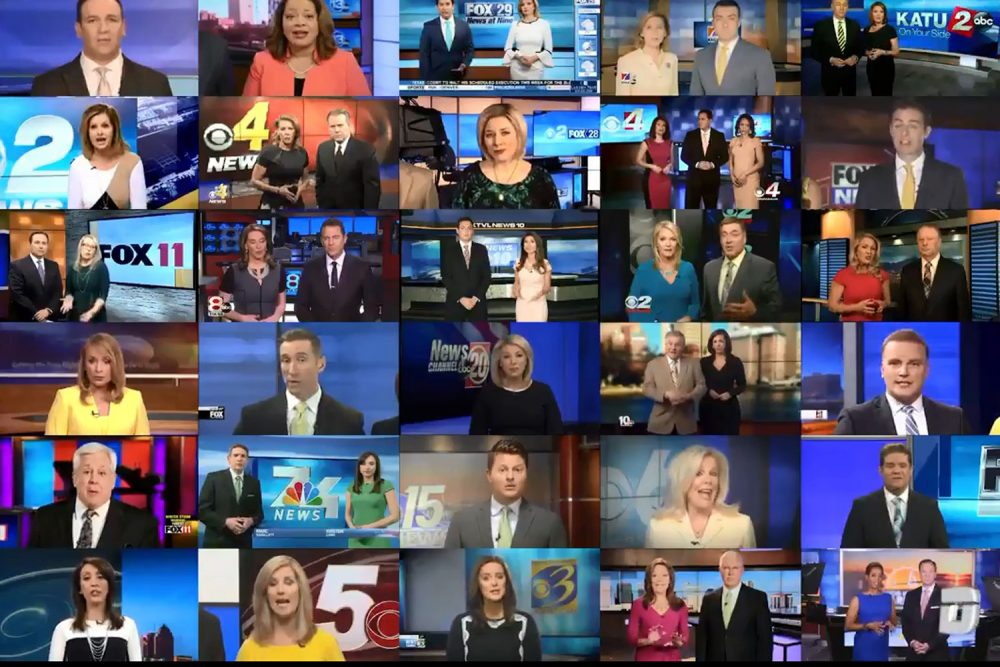
\includegraphics[width=.95\textwidth]{sinclair_cropped}
        \caption{Images from 30 of 210 Stations Reading the Script \parencite[][]{Burke_2018}}
        \end{subfigure}%
    \begin{subfigure}[bt]{.6\textwidth}
        \centering
            \begin{framed}
                \begin{quote}
                    \textbf{(A):} But we're concerned about the troubling trend of irresponsible, one sided news stories plaguing our country. The sharing of biased and false news has become all too common on social media.

                    \textbf{(B):} More alarming, some media outlets publish these same fake stories... stories that just aren't true, without checking facts first.

                    \textbf{(A):} Unfortunately, some members of the media use their platforms to push their own personal bias and agenda to control 'exactly what people think'...This is extremely dangerous to a democracy.
                \end{quote}
            \end{framed}
        \caption{Transcript of Segment \parencite[][]{Cohen_2018}}
    \end{subfigure}}\\

\end{figure}








